\documentclass{article}
\usepackage{fullpage,graphicx}
\usepackage{hyperref}
\usepackage[
  backend=bibtex,
  style=numeric,
  maxcitenames=2]{biblatex}
\addbibresource{ref}
\def\sectionautorefname{Section}
\def\subsectionautorefname{Subsection}
\def\subsubsectionautorefname{Subsubsection}
\def\lstnumberautorefname{Line}
\usepackage[dvipsnames,svgnames,x11names]{xcolor}
\usepackage{textcomp,listings,lstparams,lstcoq}
\lstdefinestyle{customcoq}{
  language=Coq,
  literate={<>}{$\ne$}1
  {->}{$\to$}1
}
\lstdefinestyle{json}{
  language=Coq,
  literate={@}{$@$}1
  {this}{$\ottkw{this}$}4
  {ref}{$\ottkw{ref}$}3
}
\newcommand{\ilc}[1]{\lstinline[style=customcoq]{#1}}
\newcommand{\ilj}[1]{\lstinline[style=json]{#1}}

\usepackage{draft} % local
\newif\ifdraft\drafttrue
\newnote{lys}{BrickRed}
\newnote{bcp}{Chocolate}
\newnote{sz}{violet}

\usepackage{amsthm,amssymb}
\theoremstyle{definition}
\newtheorem{definition}{Definition}

\newcommand{\Nat}{\mathbb N}
\newcommand{\Let}{\ottkw{let}\;}
\newcommand{\In}{\;\ottkw{in}}
\newcommand{\letin}[2]{\Let#1=#2\In}
\newcommand{\sigT}[2]{\{\exists#1\&#2\}}
\newcommand{\existT}[2]{\{*#1,#2\}}
\newcommand{\Server}{\ottkw{Server}}
\newcommand{\Validator}{\ottkw{Validator}}
\newcommand{\stepServer}{\ottkw{stepServer}}
\newcommand{\stepValidator}{\ottkw{stepValidator}}
\newcommand{\sstep}{\ottkw{sstep}}
\newcommand{\vstep}{\ottkw{vstep}}
\newcommand{\option}{\ottkw{option}\;}
\newcommand{\Some}[1]{\ottkw{Some}\;#1}
\newcommand{\None}{\varnothing}
\newcommand{\List}{\ottkw{list}\;}
\newcommand{\nil}{\varepsilon}
\newcommand{\yields}[3]{#1\overset{#2}{\longrightarrow}#3}
\newcommand{\accepts}[3]{#1\overset{#2}{\longrightarrow}#3}
\newcommand{\sound}{\ottkw{sound}}
\newcommand{\issound}[2]{#1\;\sound_{#2}}
\newcommand{\complete}{\ottkw{complete}}
\newcommand{\iscomplete}[2]{#1\;\complete_{#2}}
\newcommand{\Prog}{\ottkw{Prog}}
\newcommand{\serverOf}{\ottkw{serverOf}}
\newcommand{\validatorOf}{\ottkw{validatorOf}}
\newcommand{\Reflects}[2]{#1\sim #2}
\newcommand{\Constraint}{\ottkw{Constraint}}
\newcommand{\fresh}{\ottkw{fresh}}
\newcommand{\solvable}{\ottkw{solvable}}
\newcommand{\Write}{\ottkw{write}}
\newcommand{\Havoc}{\ottkw{havoc}}
\newcommand{\Exec}{\ottkw{exec}}
\newcommand{\If}{\ottkw{if}\;}
\newcommand{\Then}{\ottkw{then}\;}
\newcommand{\Else}{\ottkw{else}\;}
\newcommand{\bool}{\mathbb B}
\newcommand{\Assignment}{\ottkw{Assignment}}
\newcommand{\Evaluate}{\ottkw{evaluate}}
\newcommand{\Satisfy}{\ottkw{satisfy}}
\newcommand{\true}{\ottkw{true}}
\newcommand{\false}{\ottkw{false}}
\newcommand{\imp}{\ottkw{implements}}
\newcommand{\pass}{\ottkw{passes}}
\newcommand{\exhaust}{\ottkw{exhaustive}}
\newcommand{\defeq}{\triangleq}
\newcommand{\implements}[2]{#1\;\imp\;#2}
\newcommand{\passes}[2]{#1\;\pass\;#2}
\newcommand{\isexhaust}[1]{#1\;\exhaust}

% generated by Ott 0.31 from: jexp.ott
\usepackage{amsmath,amssymb}
\usepackage{supertabular}
\usepackage{geometry}
\usepackage{ifthen}
\usepackage{alltt}%hack
\geometry{a4paper,dvips,twoside,left=22.5mm,right=22.5mm,top=20mm,bottom=30mm}
\usepackage{color}
\newcommand{\ottdrule}[4][]{{\displaystyle\frac{\begin{array}{l}#2\end{array}}{#3}\quad\ottdrulename{#4}}}
\newcommand{\ottusedrule}[1]{\[#1\]}
\newcommand{\ottpremise}[1]{ #1 \\}
\newenvironment{ottdefnblock}[3][]{ \framebox{\mbox{#2}} \quad #3 \\[0pt]}{}
\newenvironment{ottfundefnblock}[3][]{ \framebox{\mbox{#2}} \quad #3 \\[0pt]\begin{displaymath}\begin{array}{l}}{\end{array}\end{displaymath}}
\newcommand{\ottfunclause}[2]{ #1 \equiv #2 \\}
\newcommand{\ottnt}[1]{\mathit{#1}}
\newcommand{\ottmv}[1]{\mathit{#1}}
\newcommand{\ottkw}[1]{\mathbf{#1}}
\newcommand{\ottsym}[1]{#1}
\newcommand{\ottcom}[1]{\text{#1}}
\newcommand{\ottdrulename}[1]{\textsc{#1}}
\newcommand{\ottcomplu}[5]{\overline{#1}^{\,#2\in #3 #4 #5}}
\newcommand{\ottcompu}[3]{\overline{#1}^{\,#2<#3}}
\newcommand{\ottcomp}[2]{\overline{#1}^{\,#2}}
\newcommand{\ottgrammartabular}[1]{\begin{supertabular}{llcllllll}#1\end{supertabular}}
\newcommand{\ottmetavartabular}[1]{\begin{supertabular}{ll}#1\end{supertabular}}
\newcommand{\ottrulehead}[3]{$#1$ & & $#2$ & & & \multicolumn{2}{l}{#3}}
\newcommand{\ottprodline}[6]{& & $#1$ & $#2$ & $#3 #4$ & $#5$ & $#6$}
\newcommand{\ottfirstprodline}[6]{\ottprodline{#1}{#2}{#3}{#4}{#5}{#6}}
\newcommand{\ottlongprodline}[2]{& & $#1$ & \multicolumn{4}{l}{$#2$}}
\newcommand{\ottfirstlongprodline}[2]{\ottlongprodline{#1}{#2}}
\newcommand{\ottbindspecprodline}[6]{\ottprodline{#1}{#2}{#3}{#4}{#5}{#6}}
\newcommand{\ottprodnewline}{\\}
\newcommand{\ottinterrule}{\\[5.0mm]}
\newcommand{\ottafterlastrule}{\\}
\newcommand{\ottmetavars}{
\ottmetavartabular{
 $ \ottmv{l} $ & \ottcom{trace labels} \\
 $ \ottmv{f} $ & \ottcom{functions} \\
 $ \ottmv{s} $ & \ottcom{string literals} \\
 $ \ottmv{i} $ & \ottcom{integers} \\
}}

\newcommand{\ottjexp}{
\ottrulehead{\ottnt{jexp}}{::=}{\ottcom{J-expressions}}\ottprodnewline
\ottfirstprodline{|}{\ottkw{ref} \, \ottmv{l} \, \ottnt{p} \, \ottmv{f}}{}{}{}{}\ottprodnewline
\ottprodline{|}{\ottsym{\{}  \ottnt{object}  \ottsym{\}}}{}{}{}{}\ottprodnewline
\ottprodline{|}{\ottsym{[}  \ottnt{array}  \ottsym{]}}{}{}{}{}\ottprodnewline
\ottprodline{|}{\ottmv{s}}{}{}{}{}\ottprodnewline
\ottprodline{|}{\ottmv{i}}{}{}{}{}\ottprodnewline
\ottprodline{|}{\ottkw{true}}{}{}{}{}\ottprodnewline
\ottprodline{|}{\ottkw{false}}{}{}{}{}\ottprodnewline
\ottprodline{|}{\ottkw{null}}{}{}{}{}}

\newcommand{\ottobject}{
\ottrulehead{\ottnt{object}}{::=}{}\ottprodnewline
\ottfirstprodline{|}{}{}{}{}{}\ottprodnewline
\ottprodline{|}{\ottsym{"}  \ottmv{s}  \ottsym{"}  \ottsym{:}  \ottnt{jexp}  \ottsym{,}  \ottnt{object}}{}{}{}{}}

\newcommand{\ottarray}{
\ottrulehead{\ottnt{array}}{::=}{}\ottprodnewline
\ottfirstprodline{|}{}{}{}{}{}\ottprodnewline
\ottprodline{|}{\ottnt{jexp}  \ottsym{,}  \ottnt{array}}{}{}{}{}}

\newcommand{\ottp}{
\ottrulehead{\ottnt{p}}{::=}{\ottcom{J-paths}}\ottprodnewline
\ottfirstprodline{|}{\ottkw{this}}{}{}{}{}\ottprodnewline
\ottprodline{|}{\ottnt{p}  \ottsym{\#}  \ottmv{i}}{}{}{}{}\ottprodnewline
\ottprodline{|}{\ottnt{p}  \ottsym{@}  \ottmv{s}}{}{}{}{}}

\newcommand{\ottgrammar}{\ottgrammartabular{
\ottjexp\ottinterrule
\ottobject\ottinterrule
\ottarray\ottinterrule
\ottp\ottafterlastrule
}}

% defnss
\newcommand{\ottdefnss}{
}

\newcommand{\ottall}{\ottmetavars\\[0pt]
\ottgrammar\\[5.0mm]
\ottdefnss}



\title{From Interaction Trees to Asynchronous Tests}
\author{Yishuai Li}
\begin{document}
\maketitle
\section{Introduction}
Importance of rigorous testing in software development.

Main challenge: nondeterminism in various parts of the system.

Goal: a systematic testing framework for networked systems, addressing internal
nondeterminism and network nondeterminism.

Methodology: interpret model specification into testing logic; introduce
abstract representation for test input generation and shrinking.

Broader impact: Handling network nondeterminism is the first step towards
testing generic concurrent systems.  Automatically deriving tests from formal
specifications enables iterative incremental development of reliable software.

Todo thesis claim.  What technology solves what problem.

5--6 pages.

\section{Background}
Property-based testing with QuickCheck.  Limitation: nondeterminism makes
validation logic hard to write.

ISSTA related work.

5--6+ pages.

\section{Prior Results}
Model-based testing in ISSTA paper.

Refactor previous paper.

\subsection{Theories of Interactive Testing}
{\em Interactive testing} is a process that reveals the SUT's interactions and
determines whether it satisfies the specification.  There are two kinds of
interactions: (1) {\em inputs} that the tester can specify, and (2) {\em
  outputs} that are observed from the SUT.  In particular, when testing
networked systems, the input is a message sent by the tester, and the output is
a message received from the SUT.

When viewing the SUT as a function from inputs to outputs, we can test the
system by (1) providing an input, (2) get the output, and (3) validating the
input-output pair.  This process is called {\em synchronous testing}.

However, the nature of networked systems is that multiple messages might arrive
at the system simultaneously, and a high-throughput system should handle the
messages concurrently.  To check the system's validity upon concurrent inputs,
the tester should send multiple messages, rather than executing ``one client at
a time''.  This non-blocking process is called {\em asynchronous testing}.

My goal is to formalise the techniques in \textcite{li2021modelbased} into a generic
theory for asynchronous testing.  I start by formalising synchronous testing
theory, which describes how to build a sound and exhaustive tester, and will
expand the theory to asynchronous testing.

A tester consists of two parts: (i) a test harness that interacts with the SUT
and observes the interactions, and (ii) a validator that determines whether the
observations satisfy the specification.

The test harness needs to produce counterexamples effectively, and provide good
coverage of test cases.  The goal is to locate unknown bugs within a fixed
budget, which is more practical than theoretical, and will be discussed in
\autoref{sec:harness}.  The test theory in this dissertation focuses on
guaranteeing the soundness and completeness of the validator logic.

\subsubsection{Synchronous Testing Language}

\paragraph{Server specifications and validator implementations}
Synchronous testing can be viewed as a {\em server} interacting with a single
client, producing a {\em trace} of queries and responses, and a validator
determing whether the trace is acceptable or not.

\begin{definition}[Server model]
Let $Q$ be the query type, $A$ be the response type, $S$ be some server state,
then a deterministic server starts from an initial state, takes a query,
computes the response based on its current state, computes the next server
state, and loops over:
\[ \ottkw{DeterministicServer}\triangleq\sigT{S}{(Q \times S \to A \times S) \times S} \]

In general, servers have {\em internal nondeterminism} that allows the responses
and transitions to depend on internal choices that are invisible to the testers
{\it e.g.} timestamps and hash algorithms.  Let $C$ be the space of internal
choices, then a nondeterministic server is specified as:
\begin{align*}
  \Server\triangleq\sigT{S}{(&Q \times C \times S \to A \times S) \times S} \\
  \stepServer :\quad&Q\times C \times \Server \to A\times \Server \\
  \stepServer(q,c,\existT{S}{(\sstep, state)})\triangleq\;&\letin{(a,state')}{\sstep(q,c,state)} \\
  &(a, \existT{S}{(\sstep, state')})
\end{align*}
\end{definition}

\begin{definition}[Validator]
Let $V$ be some validator state, then a validator starts from an initial state,
takes a query and its corresponding response, determines whether these
interactions are valid, and computes the next validator state upon valid:
\begin{align*}
  \Validator\triangleq\sigT{V}{(&Q \times A \times V \to \option V) \times V} \\
  \stepValidator:\quad&Q\times A \times \Validator \to \option \Validator \\
  \stepValidator(q,a,\existT{V}{(\vstep, state)})\triangleq\;&\begin{cases}
  \Some{\existT{V}{(\vstep,state')}} & \vstep(q,a,state)=\Some{state'} \\
  \None & \vstep(q,a,state)=\None
  \end{cases}
\end{align*}
\end{definition}

\paragraph{Deriving validator from server definition}
While it is possible to write server specifications and validators manually,
\textcite{li2021modelbased} have shown that internal nonderminism makes the
validator difficult to implement and reason about, and demonstrated how to
automatically derive a validator from a server specification.  That paper has
evaluated the derived validator's effectiveness by finding bugs in real world
programs, but did not provide a mathematical proof.  To construct a generic
derivation process, I start with a simplified derivation model for synchronous
tests.

\begin{definition}[Server and validator of a program]
  A program $p\in\Prog$ is a representation that can be ``instantiated'' into a
  server model:
  \[ \serverOf:\Prog\to\Server \]
  A program can also be ``interpreted'' into a validator:
  \[ \validatorOf:\Prog\to\Validator \]
\end{definition}

\paragraph{Soundness and completeness}
A tester is {\em sound} if any valid implementation passes it {\it i.e.} no
false rejection.  A tester is {\em exhaustive} if any invalid implementation
fails it (given sufficient time) {\it i.e.} no false acceptance.

A sound tester requires a sound validator, and a faithful test harness
that correctly interprets its observed behavior into the validator's input; An
exhaustive tester requires a {\em complete} validator, a faithful test harness,
plus an exhaustive test input generator that reveals all possible behavior of
the SUT.  Here I focus on the soundness and completeness of the validator.

\begin{definition}[Trace validity]
  A trace is valid if there exists an execution of the server model that {\em
    yields} it.  Let the trace be a list of query-response pairs $(\List
  (Q\times A))$, then:
  \begin{enumerate}
  \item Any server can step to itself, yielding an empty trace:
    \[\forall s\in\Server, \yields{s}{\nil}{s}\]
  \item A server yields a non-empty trace if it can yield the head of the trace
    and step into a server that yields the tail of the trace:
    \begin{align*}
      &\forall s,s_2\in\Server,\forall l\in\List(Q\times A),\forall q\in Q,\forall a\in A,\\
      &(\exists s_1\in\Server,\exists c\in C\mid\yields{s}{l}{s_1}\wedge
      \stepServer(q,c,s_1)=(a,s_2)) \\
      &\implies \yields{s}{l+(q,a)}{s_2}
    \end{align*}
  \end{enumerate}
\end{definition}

\begin{definition}[Trace acceptance]
  A trace is {\em accepted} by a validator if the validator consumes the entire
  trace and steps into a nonempty state:
  \begin{enumerate}
  \item Any validator accepts an empty trace and steps to itself:
    \[ \forall v\in\Validator,\accepts{v}{\nil}{v} \]
  \item A validator accepts a non-empty trace if it can consume the head of the
    trace and step into a validator that accepts the end of the trace:
    \begin{align*}
      &\forall v,v_2\in\Validator,\forall
      l\in\List(Q\times A),\forall q\in Q, \forall a\in A, \\
      & (\exists v_1\in\Validator\mid\accepts{v}{l}{v_1}\wedge
      \stepValidator(q,a,v_1)=\Some{v_2}) \\ &\implies
      \accepts{v}{l+(q,a)}{v_2}
    \end{align*}
  \end{enumerate}
\end{definition}

\begin{definition}[Soundness]
  A validator is {\em sound} per server specification if it accepts all valid
  trace of the specification:
  \[ \issound{v}{s}\triangleq\forall l\in\List(Q\times A),(\exists s'\in\Server\mid\yields{s}{l}{s'})\implies\exists v'\in\Validator\mid\accepts{v}{l}{v'} \]
\end{definition}

\begin{definition}[Completeness]
  A validator is {\em complete} per server specification if it only accepts valid
  traces of the specification:
  \[ \iscomplete{v}{s}\triangleq\forall l\in \List(Q\times A),(\exists{v'}\in\Validator\mid\accepts{v}{l}{v'})\implies\exists{s'}\in\Server\mid\yields{s}{l}{s'} \]
\end{definition}

\subsubsection{Reasoning on Synchronous Testers}
\label{sec:sync-reasoning}

Given a server $\existT{S}{(\sstep, s_0)}$ and a validator
$\existT{V}{(\vstep,v_0)}$, to prove its soundness and completeness, we need to
show properties over the step functions and the initial states.

\paragraph{Proving completeness}
The validator's completeness says: For any trace accepted by the validator,
there exists an execution of the server specification that yields this trace.

Since the server and validator are both loops, I introduce an invariable
$\{\Reflects{v}{s}\mid v\in V,s\in S\}$, which is preserved by the loops' step
functions.  The completeness proof is by induction of the validation path, and
construct the corresponding server execution path based on the following
assumptions:

\begin{enumerate}
\item Any accepting validator step has some server state that reflects the
  post-validation state:
  \begin{align*}
    \forall q\in Q,\forall a\in A,\forall v, v'\in V,\;&\vstep(q,a,v)=\Some{v'}\\
    &\implies\exists s'\in S,\Reflects{v'}{s'} 
  \end{align*}
\item Any accepting validator step whose post-validation state reflects some
  post-execution server state has a corresponding server step from a
  pre-execution state that reflects the pre-validation state:
  \begin{align*}
    &\forall q\in Q,\forall a\in A,\forall v,v'\in V,\forall s'\in S,\\
    &\vstep(q,a,v)=\Some{v'}\wedge\Reflects{v'}{s'}\\
    &\implies\exists c\in C,\exists s\in S,\sstep(q,c,s)=(a,s')\wedge\Reflects{v}{s}
  \end{align*}
\item The initial validator state only reflects the initial server state:
  \[\{s\mid\Reflects{v_0}{s}\}=\{s_0\}\]
\end{enumerate}

\subsubsection{Case Study: Single Instruction Server}

In this experiment, I'll propose simple server language where the program is a
single instruction.  I'll then show how to instantiate the program into a server
model, and how derive the program into a validator that is sound and complete.
That is, defining $\serverOf$ and $\validatorOf$ functions for $\Prog$ such
that:

\begin{align*}
  \forall p:\Prog,\;&\letin{s}{\serverOf(p)}\\
  &\letin{v}{\validatorOf(p)}\\
  &\issound{v}{s}\wedge\iscomplete{v}{s}
\end{align*}

\paragraph{Server language}
The server stores a key-value mapping $K\to\Nat$.  The server program is a
three-address instruction that performs an arithmetic operation:
\[\Prog \triangleq \{!dst\gets !src_1\;op\;!src_2\mid op\in\{+,-,\times,\div\};
dst,src_1,src_2\in K\}\]

A program in this language is instantiated into a server step as follows: Upon
receiving a query $q\in Q$, the server writes a choice $c\in C$ to key 1, and
writes the query to key 0.  The server then runs the instruction, and sends back
the value stored in key 0:

\begin{align*}
  \rlap{$Q\triangleq\Nat\qquad C\triangleq\Nat\qquad A\triangleq\Nat$}\\
  \rlap{$\serverOf(p)\triangleq\existT{(K\to\Nat)}{(\sstep(p), (\_\mapsto0))}$}\\
  \rlap{where}\\
  \rlap{$\sstep(!dst\gets !src_1\;op\;!src_2)(q,c,s_0)\triangleq$}\\
  &\qquad\letin{s_1}{s_0 [k_1\mapsto c]}\\
  &\qquad\letin{s_2}{s_1 [k_0\mapsto q]}\\
  &\qquad\letin{s_3}{s_2 [dst\mapsto s_2(src_1)\;op\;s_2(src_2)]}\\
  &\qquad(s_3(k_0), s_3)
\end{align*}

To check a trace against this server model, the validator introduces symbolic
variables $x\in X$ to represent the values stored in each key.  The validator
also maintains a set of constraints that reflect the server's computations:

\begin{align*}
  \rlap{$E\triangleq\; \Nat \cup \{!x\mid x\in X\} \cup \{!x_1\;op\;!x_2\mid
    op\in\{+,-,\times,\div\}; x_1,x_2\in X\}$}\\
  \rlap{$\Constraint\triangleq\{e_1=e_2\mid e_1,e_2\in E\}$}\\
  \rlap{$V\triangleq(K\to X)\times\List\Constraint$}\\
  \rlap{$\validatorOf(p)\triangleq\existT{V}{(\vstep(p), ((\_\mapsto x_0),(0=\;!x_0)))}$}\\
  \rlap{where}\\
  \rlap{$\vstep(p)(q,a,v_0)\triangleq\;$}\\
  &\qquad\letin{v_1&}{\;&\Havoc(k_1,v_0)&}\\
  &\qquad\letin{v_2&}{\;&\Write(k_0,q,v_1)&}\\
  &\qquad\letin{(vs_3,cs_3)&}{\;&\Exec(p,v_2)&}\\
  &\qquad\letin{cs_4&}{\;&cs_3+(!vs_3(k_0)=a)&}\\
  \rlap{$\qquad\If \solvable(cs_4)\;\Then \Some{(vs_3,cs_4)}\;\Else \None$}\\
  \rlap{$\Write(k,q,(vs,cs))\triangleq$}\\
  \rlap{$\qquad\letin{x}{\fresh(vs,cs)}$}\\
  \rlap{$\qquad(vs[k\mapsto x],cs+(q=\;!x))$}\\
  \rlap{$\Havoc(k,(vs,cs))\triangleq$}\\
  \rlap{$\qquad\letin{x}{\fresh(vs,cs)}$}\\
  \rlap{$\qquad(vs[k\mapsto x],cs)$}\\
  \rlap{$\Exec((!dst\gets\;!src_1\;op\;!src_2),(vs,cs))\triangleq$}\\
  \rlap{$\qquad\letin{x}{\;\fresh(vs,cs)}$}\\
  \rlap{$\qquad(vs[dst\mapsto x],cs+(!vs(src_1)\;op\;!vs(src_2)=\;!x))$}\\
  \rlap{$\fresh:V\to X$}\\
  \rlap{$\solvable:\List\Constraint\to\bool$}
\end{align*}

When the $\sstep$ function modifies the server state, the $\vstep$ function
updates the validator's view of the server correspondingly: When the server
stores a query to key 0, the $\Write$ function maps key 0 to a $\fresh$
variable, and adds a constraint that the variable's value is equal to the query.
When the server stores an internal choice to key 1, the $\Havoc$ function maps
key 1 to a fresh variable with no constraints, because its exact value is
invisible to the validator.  When the server runs a three-address instruction,
the $\Exec$ function maps the destination to a fresh variable, and adds a
constraint that the variable's value should reflect the three-address
computation.

After updating its symbolic view of the server, the validator expects the
observed response to be explainable by its symbolic view.  Such expectation is
checked by a constraint solver, that determines whether the constraints can be
satisfied by some assignment of the variables:

\begin{align*}
  \Assignment\triangleq\;&X\to\Nat\\
  \Evaluate\quad:\;&\Assignment\times E\to\Nat\\
  \Satisfy(asgn,cs)\triangleq\;&\forall (e_1=e_2)\in cs,\\
  &\Evaluate(asgn,e_1)=\Evaluate(asgn,e_2)\\
  \forall cs\in\List{\Constraint},\;&\solvable(cs)\\
  &\iff\exists\; asgn\in\Assignment,\Satisfy(asgn,cs)
\end{align*}

To prove the validator's completeness, the reflection relation is defined as:

\begin{align*}
  (\Reflects{(vs,cs)}{s})\triangleq\exists\;asgn,\;&\Satisfy(asgn,cs)\\
  &\wedge \forall k\in K,asgn(vs(k))=s(k)
\end{align*}

This reflection definition is sufficient for proving the validator's
completeness, as it satisfies all the assumptions in \autoref{sec:sync-reasoning}:

\begin{enumerate}
\item Any accepting validator step has solved the post-validation constraints
  $cs'$, which implies an assignment $asgn$ that satisfies $cs'$.  Let $vs'$ be
  the post-validation key-variable mapping, then $s'=asgn\circ vs'$ reflects the
  post-validation state $(vs',cs')$ by definition.

\item The $\vstep$ function monotonically increases the list of constraints, and
  thus monotonically narrows the space of satisfying assignments.  Let $s'$ be
  the post-execution server state that reflects the post-validation state
  $(vs',cs')$, then $asgn$ is guaranteed to satisfy the pre-validation
  constraints $cs$.  Therefore, by analysing the execution of
  $\vstep(q,a,(vs,cs))$, we can construct the pre-execution server state
  $s=asgn\circ vs$ and the server's internal choice $c=asgn(\fresh(vs,cs))$ that
  satisfy $\sstep(q,c,s)=(a,s')$ and $\Reflects{(vs,cs)}{s}$.

\item From the definition of the server and validator's initial state, we can
  show that the initial server state is the only state that reflects the initial
  validator state.
\end{enumerate}

\section{Research Plan}

\subsection{Theories of Interactive Testing}

\subsubsection{Synchronous Testing in General}
\subsubsection{Asynchronous Testing}

\subsection{Test Input Generation and Shrinking Techniques}
\label{sec:harness}
To make a sound and exhaustive tester useful in software engineering practices,
we need to (1) generate test inputs that can reveal potential bugs quickly, and
(2) report minimal counterexamples to debuggers, rather than thousand-line logs.

One challenge for random testing is that, to find failing examples efficiently,
it is important to generate fairly large test cases.  But then, after a failing
test case has been found, it is important to \textit{minimize} the test input to
eliminate the parts that are not relevant to provoking the failure.  Tools like
QuickCheck therefore provide automatic methods for minimizing, or {\em
  shrinking}, failing tests, by incrementally generating smaller variants until
they reach a local minimum---a counterexample that cannot be reduced any
further.

Traditional shrinking doesn't work well for impure programs, which might mutate
state or interact with their environments, because an interesting test input in
one execution might become trivial or irrelevant in another run.  In particular,
when testing an interactive program, interesting test inputs might depend on
existing observations of the program's behavior.

To generate and shrink inputs that are interesting among different executions,
\textcite{Hughes2007} introduced a method that relates inputs to runtime
observations.  In this framework, the tester interacts with the system under
test (SUT) via function calls, and maintains a runtime state that is updated
after each call returns.  Test inputs are represented in an abstract language
that depends on the runtime state {\it e.g.} ``call function \ilc{foo(x)}, where
\ilc{x} is the return value of the 10th function call''.  Such abstract
representation is instantiated into a concrete input during runtime, by
remembering the 10th call's return value \ilc{a} to build the actual function
call \ilc{foo(a)}.

This methodology has achieved good results in testing state
machines~\cite{Hughes2016}, but the specification language requires the
interactions to be synchronous {\it i.e.} to return immediately upon call.
However, when testing networked systems, requests and responses might be delayed
or reordered \textit{en route}.  Such a scenario requires a different
specification language that allows asynchronous
interactions~\cite{li2021modelbased}, introducing new challenges in minimizing
test inputs, {\it e.g.} when a dependent response has not arrived.

I'll propose a generic method for generating and minimizing asynchronous test
interactions, by combining the idea of abstract input representation
from~\textcite{Hughes2007} with the asynchronous specification language
of~\textcite{li2021modelbased}.  The tester records a {\em trace} of network
packets sent and received, and uses the trace to instantiate abstract inputs
into concrete requests to send.  The key inovation is an intermediate
representation (IR) between structured application messages and bytes.  The IR
allows the generated abstract input to refer to specific fields in the trace,
and can handle situations where the referred field is absent (caused by internal
or network nondeterminism).

\subsubsection{Overview}
\begin{figure}
  \centering
  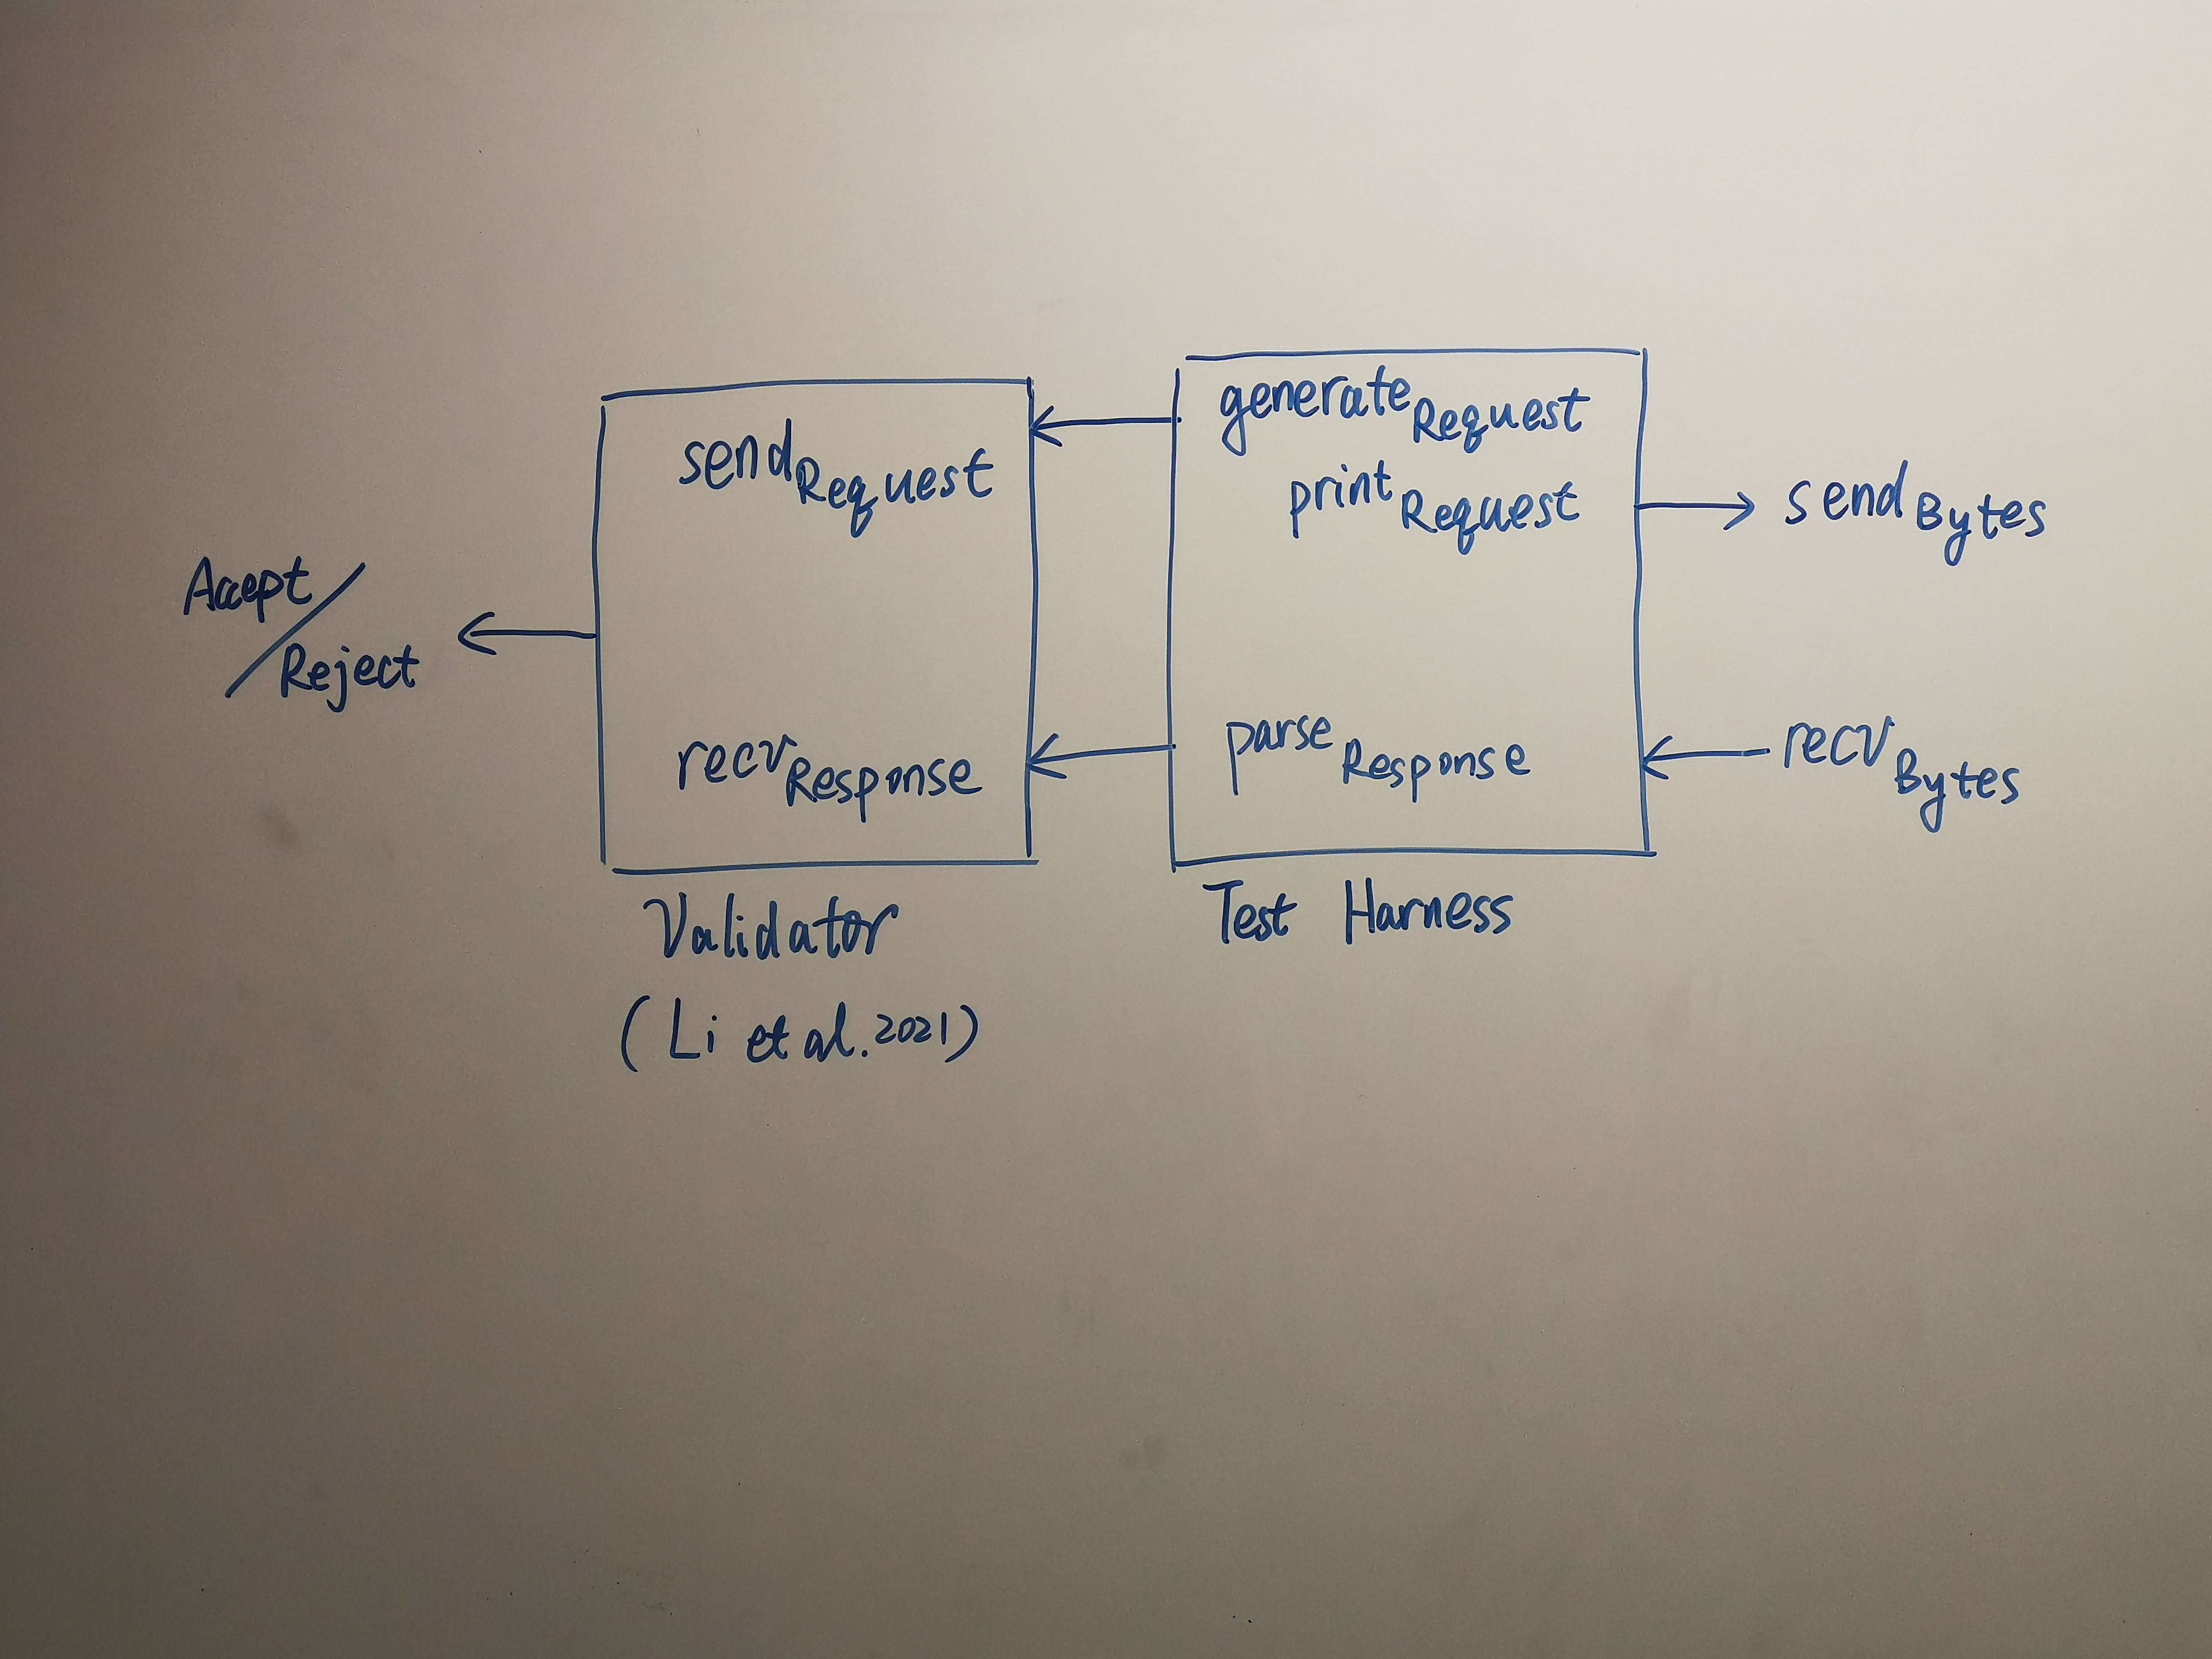
\includegraphics[width=.9\textwidth]{figures/overview}
  \caption{Test framework overview}
  \label{fig:overview}
\end{figure}

As shown in \autoref{fig:overview}, the test framework consists of a {\em
  validator} that determines whether the SUT's behavior satisfies the
specification, and a {\em test harness} that provides test inputs for the
validator.

A {\em validator} is a client-side model program that observes messages sent and
received and decides whether these interactions are conformant to the
specification.  For example, a simple validator for echo server is written as:
\begin{lstlisting}[style=customcoq]
  let validateEcho =
    request := sendRequest();
    response := recvResponse();
    if response <> request
    then reject
    else validate
\end{lstlisting}
Notice that the \ilc{sendRequest} event does not take the request to be sent as
argument, but in stead returns the request actually sent.  The validator only
describes the logic that checks messages sent and received, while the test
harness computes what requests to send.

The {\em test harness} takes a validator and turns it into an executable program
that performs network interactions.  It handles the validator's send and receive
events, and generates the requests to be sent.  A simple test harness for the
validator above is written as:
\begin{lstlisting}[style=customcoq]
  let execute(v) =
    match v with
    | x := sendRequest(); v'(x) =>
      request := arbitraryRequest();
      sendBytes(print(request));
      execute(v'(request))
    | x := recvRequest(); v'(x) =>
      responseBytes := recvBytes();
      execute(v'(parse(responseBytes)))
    | reject => reject
    end in
  execute(validateEcho)
  (* ... is equivalent to ... *)
  let executeValidateEcho =
    request := arbitraryRequest();
    sendBytes(print(request));
    responseBytes := recvBytes();
    if parse(responseBytes) <> request
    then reject
    else executeValidateEcho
\end{lstlisting}

The \ilc{arbitraryRequest} generator here produces requests randomly.  To
generate requests that depend on previously observed messages, my framework will
extend the test harness in \autoref{fig:overview} that records a trace of
messages.

\subsubsection{Architecture}
\begin{figure}
  \centering
  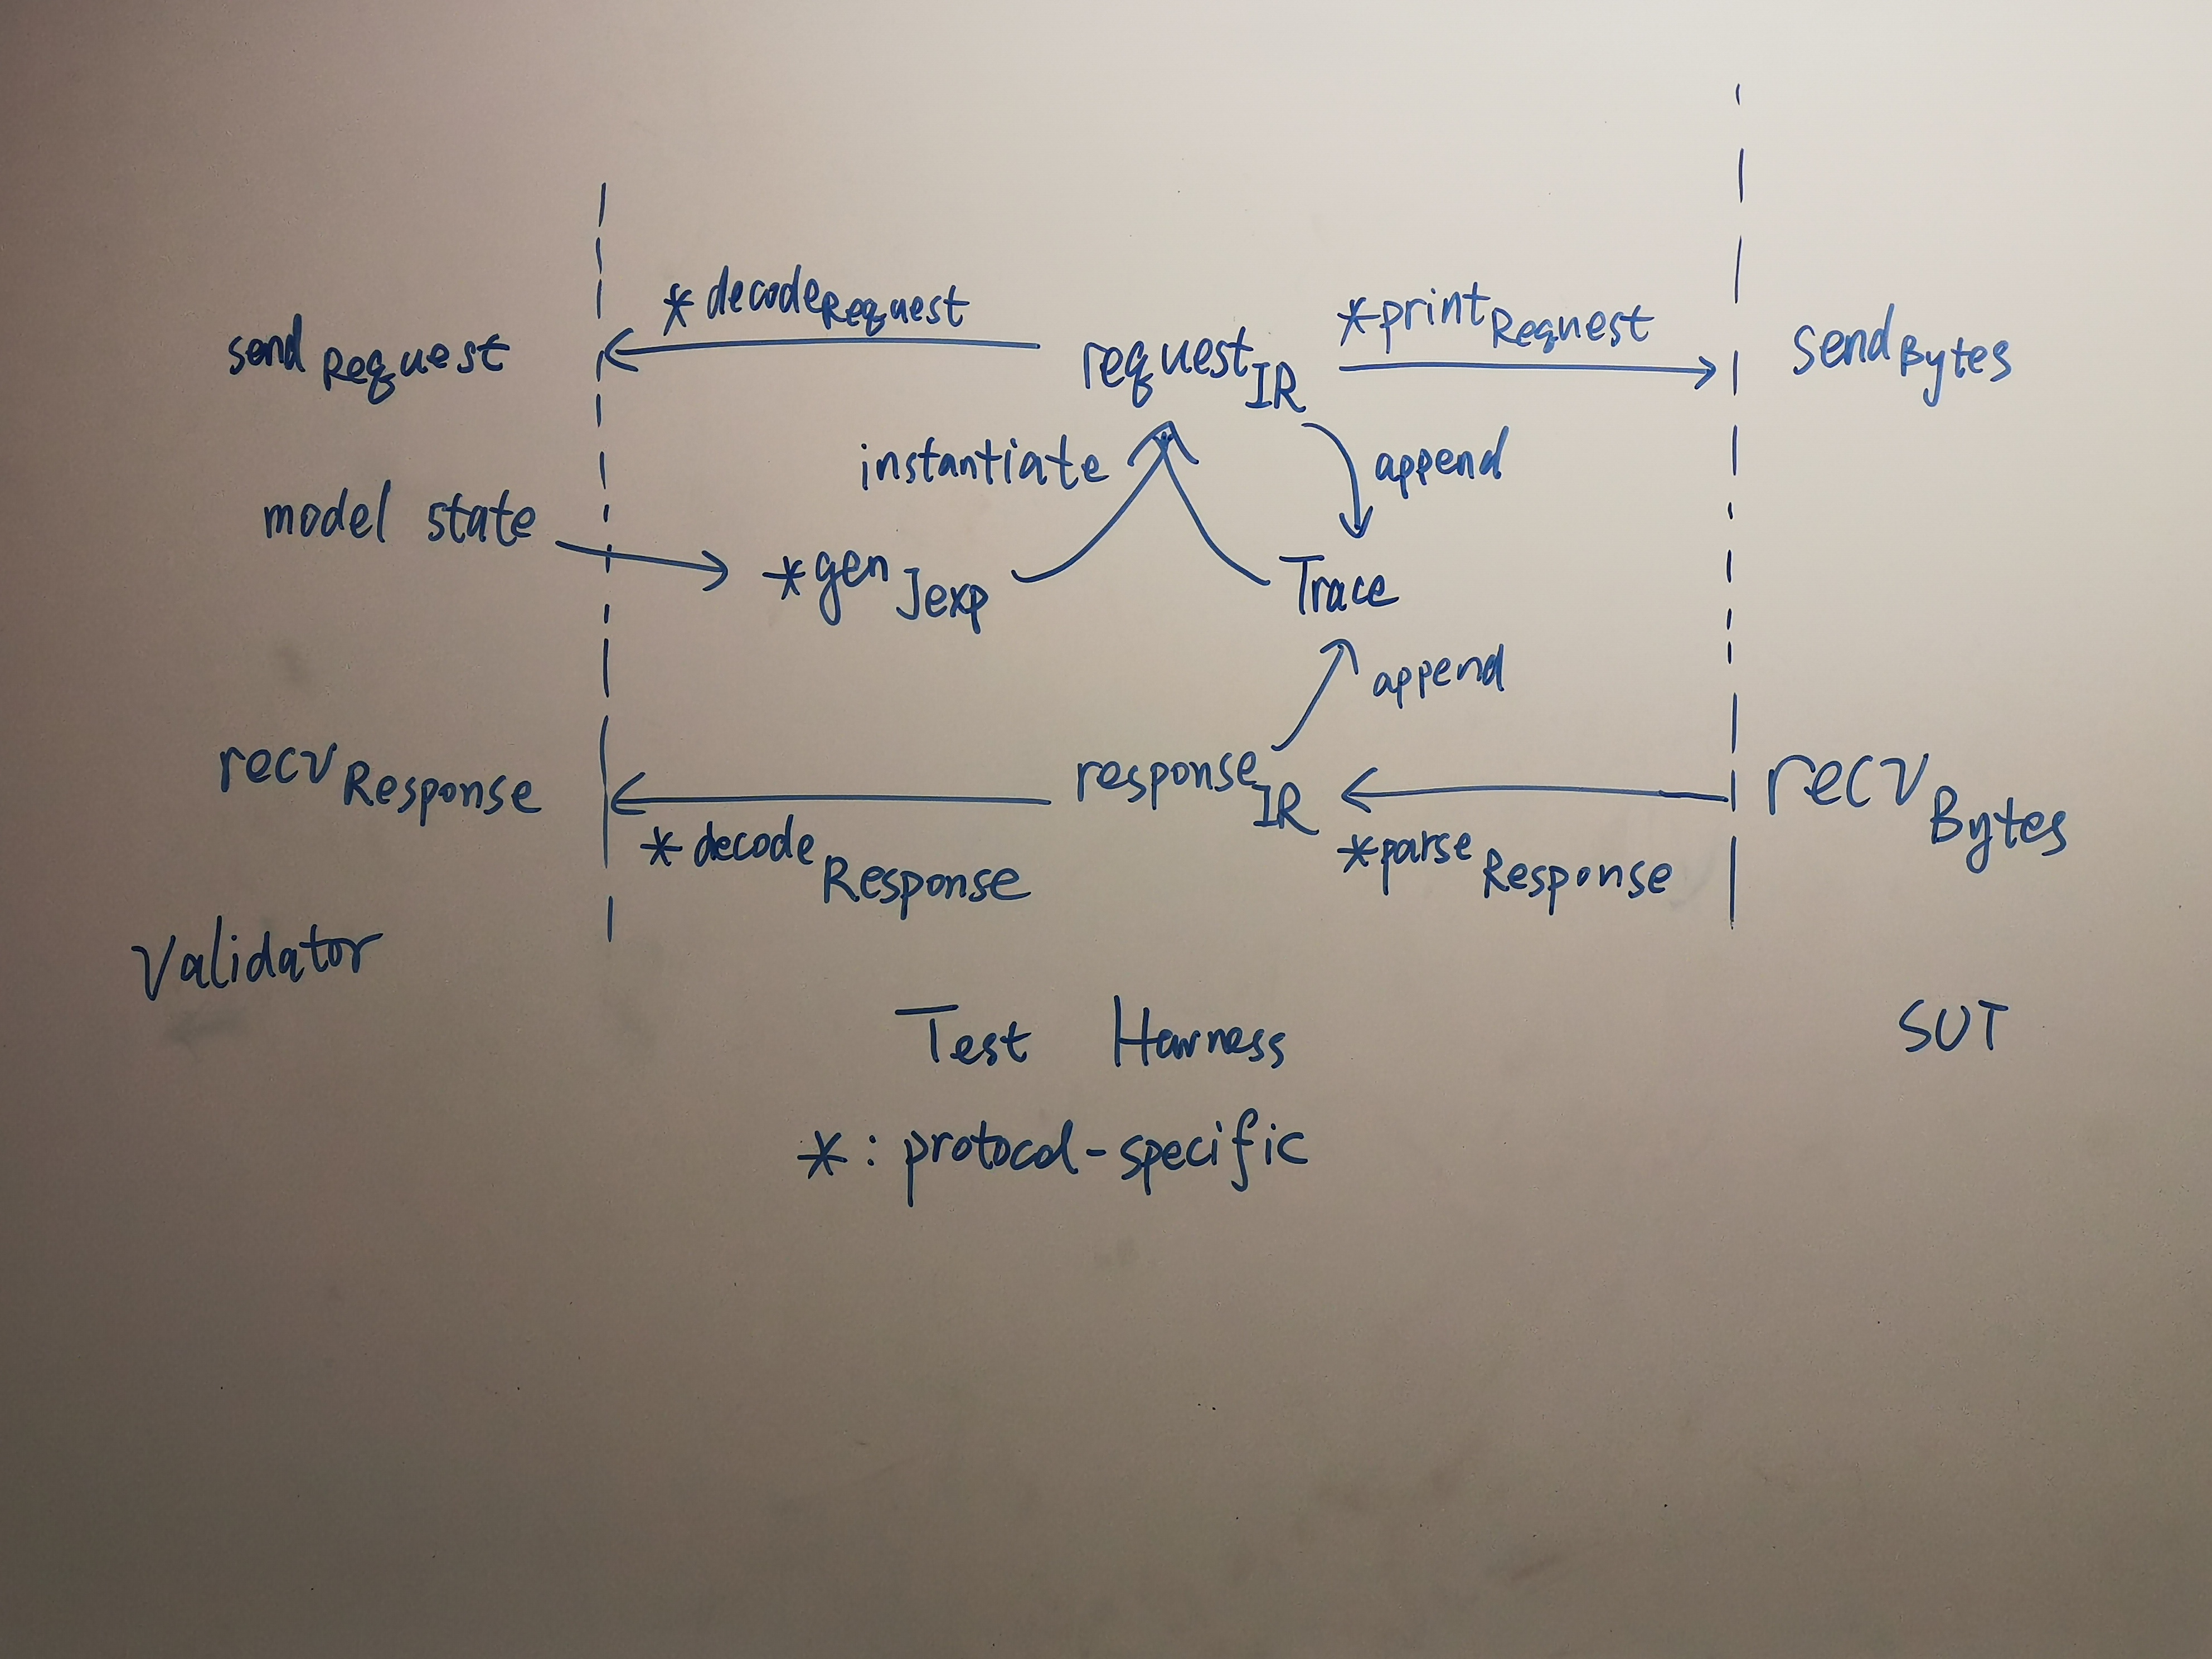
\includegraphics[width=.8\textwidth]{figures/harness}
  \caption{Test harness mechanism}
  \label{fig:harness}
\end{figure}

As shown in \autoref{fig:harness}, the test harness records a trace of requests
and responses, using an generic intermediate representation.  Requests are
generated as ``J-expressions'' that can be instantiated into a request IR based
on the trace.  For each protocol to test, the developers need to specify how to
generate J-expressions that represent requests.  Developers also need to define
how to interpret among the IR, bytes, and application messages.

\subsubsection{Intermediate representation language}
The purpose of introducing an IR in this framework is to enable a generic method
for generating requests that refer to specific fields in the trace.  For
example, when testing conditional HTTP requests, the generator wants to include
``a precondition that uses the ETag field of a previous response''; when testing
an online store, the generator wants to provide ``an order ID that the server
has mentioned before''.

I choose JSON as the intermediate representation.  Since JSON itself is widely
used in web applications, the IR should provide the flexibility for developers
to refer to any field in a JSON message, which might involve arbitrarily deep
path down the syntax tree.  \autoref{fig:ir} shows the intermediate
representation for two protocols.

\begin{figure}
  \begin{lstlisting}[style=customcoq]
    Example response1 : http_response :=
      Response (Status (Version 1 1) 200 (Some "OK"))
               [Field "ETag" "tag-foo";
                Field "Content-Length" "11"]
               (Some "content-bar").

    Example response2 : store_response :=
      Response__ListOrders [(233, (12, 100, 34, 500));
                            (996, (56, 400, 78, 20))].
  \end{lstlisting}
  \begin{minipage}[t]{.4\textwidth}
    \begin{lstlisting}[style=json]
      {
        "version": {
          "major": 1,
          "minor": 1
        },
        "code": 200,
        "reason": "OK",
        "fields": {
          "ETag": "tag-foo",
          "Content-Length": "11"
        },
        "body": "content-bar"
      }
    \end{lstlisting}
  \end{minipage}%
  \begin{minipage}[t]{.4\textwidth}
    \begin{lstlisting}[style=json]
      {
        "code": 200,
        "orders": [
          {
            "ID": 233,
            "BuyerID": 12,
            "BuyAmount": 100,
            "SellerID": 34,
            "SellAmount": 500
          },
          {
            "ID": 996,
            "BuyerID": 56,
            "BuyAmount": 400,
            "SellerID": 78,
            "SellAmount": 20
          }
        ]
      }
    \end{lstlisting}
  \end{minipage}
  \caption{Application message example for HTTP and online store protocols, and
    their corresponding intermediate representation}
  \label{fig:ir}
\end{figure}

To represent the correspondence between requests and responses, the trace labels
each message, and the request-response pair have the same label.
\autoref{fig:trace} shows a trace of messages sent and received by the tester
client.

\begin{figure}
  \begin{minipage}{.5\textwidth}
    \begin{lstlisting}[style=json]
      [
        {
          "label": 10,
          "message": {
            "method": "GET",
            "path": "index.html"
          }
        },
        {
          "label": 20,
          "message": {
            "method": "DELETE",
            "path": "index.html"
          }
        },
        {
          "label": 20,
          "message": {
            "code": 204,
            "reason": "No Content",
          }
        },
        {
          "label": 10,
          "message": {
            "code": 410,
            "reason": "Gone"
          }
        }
      ]
    \end{lstlisting}
  \end{minipage}%
  \begin{minipage}{.5\textwidth}
    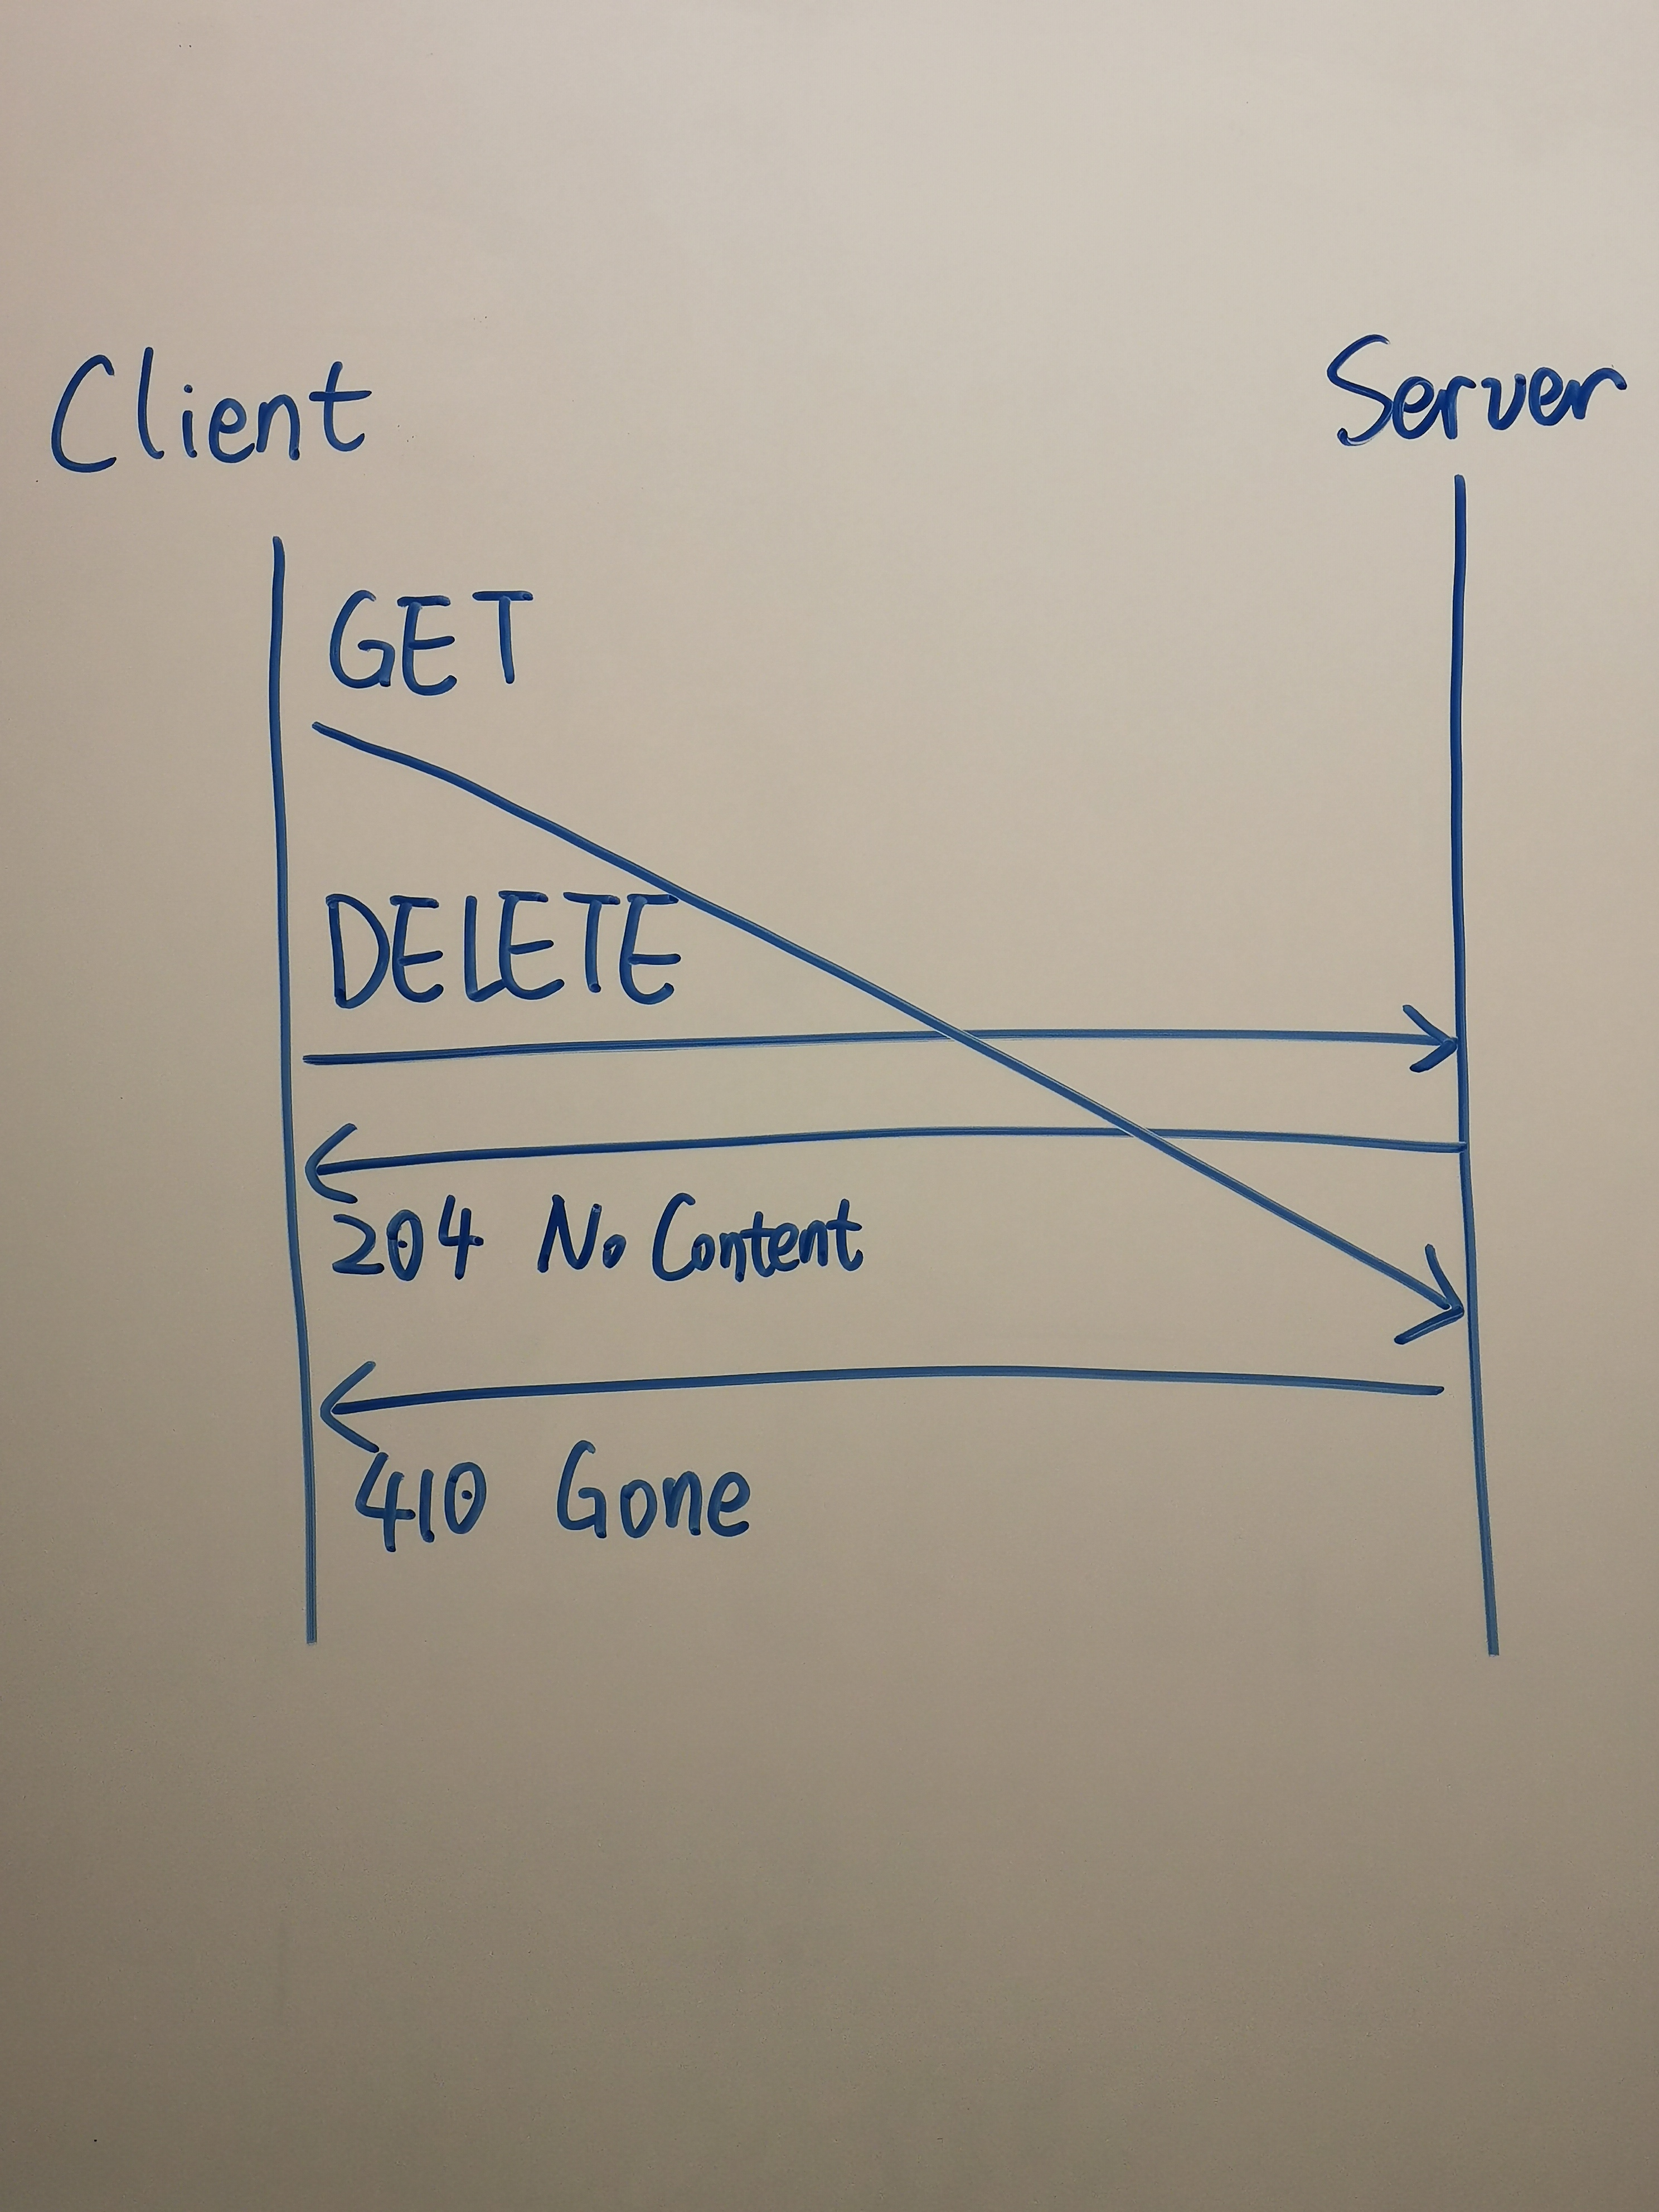
\includegraphics[width=\textwidth]{figures/trace}
  \end{minipage}
  \caption{Example client-side trace and its corresponding IR}
  \label{fig:trace}
\end{figure}

\begin{figure}
  \ottall
  \caption{Formal definition of J-expressions}
  \label{fig:jexp}
\end{figure}

Based on this unified structure of messages, I introduce a symbolic language for
representing requests, called ``J-expressions'', defined in \autoref{fig:jexp}.
The J-expression is similar to JSON, except that it allows a pointer notation
that refers to the trace.  For example, the following J-expression represents a
\ilc{takeOrder} request whose order ID is equal to the second order's ID in the
message labelled 30:
\begin{lstlisting}[style=json]
  {
    "method": "takeOrder",
    "user": 2,
    "order": ref 30 (this@"orders"#2@"ID") id
  }
\end{lstlisting}

Notice the \ilc{ref} in the final line: The first argument 30 is the message
label in the trace.  The following \ilj{this@"orders"#2@"ID"} is a path for the
generator to search in the IR, pronounced ``the `ID' field in the 2nd entry of
the array named `orders' ''.  The last argument is the transformer function that
maps the found field to the generated request, here \ilj{id} is the identical
function, meaning the found order ID is used in the result request verbatim.

Suppose a trace contains a message labelled 30, and its payload is the second
example in \autoref{fig:ir}, then the request generator can find the
corresponding order ID in the request {\it i.e.}  996, and construct the
following request IR based on the J-expression above:

\begin{lstlisting}[style=json]
  {
    "method": "takeOrder",
    "user": 2,
    "order": 996
  }
\end{lstlisting}

\subsubsection{Instantiating J-expression into request IR}
Suppose the test developer has generated some J-expression to represent request
to send, the tester harness needs to instantiate the J-expression into the
request IR.  In particular, \ilj{ref} expression referrs to a field in the
trace, so the test harness should locate its corresponding value.

When testing networked systems, response packets might be delayed by the
network.  As a result, when the tester wants to send a request that depends on a
response labelled $l$, it is possible that the response hasn't arrived yet.  In
this case, to avoid blocking the program, the test harness should find some
fallback options to instantiate the J-expression.  A useful solution is to
ignore the label and find if any message in the trace has a field of the given
J-path.  \lys{My implementation is highly functional.  Translate into imperative
  pseudocode here?}

Even if the labelled response has arrived, considering internal nondeterminism,
the response might not have a field of the given J-path {\it e.g.}  the
J-expression doesn't have a second entry in the \ilj{"orders"} array.  In this
case, the test harness can ignore the index and pick any entry in the array as
fallback.

\subsubsection{Completeness of test suite}

\begin{definition}[Specification, implementation, and test suite]
  An implementation $i:I$ is a software that performs some observable behavior.
  A specification $s:S$ is a language of valid behavior.  A test suite $t:S\to
  I\to\bool$ is a program that executes an implementation and computes whether
  its observed behavior is included in the specification.
\end{definition}

\begin{definition}[$\pass$ and $\imp$ relations]
  An implementation $\pass$ a test suite if the test suite determines that its
  behavior is included in the specification:
  \[ \passes{i}{t_s}\defeq t_s(i)=\true \]
  An implementation $\imp$ a specification if all its observable behavior is
  included in the specification:
  \[ \implements{i}{s}\defeq\forall t,t_s(i)=\true \]
\end{definition}

\begin{definition}[Soundness, exhaustiveness, and completeness]
  A test suite is $\sound$ if all implementations that $\imp$ the specification
  $\pass$ it:
  \[ \issound{t}\defeq\forall s,\forall i,
  \implements{i}{s}\implies\passes{i}{t_s} \]

  A test suite is $\exhaust$ if all implementations that $\pass$ it $\imp$ the
  specification:
  \[ \isexhaust{t}\defeq\forall s,\forall i,
  \passes{i}{t_s}\implies\implements{i}{s} \]

  A test suite is $\complete$ if it's both $\sound$ and $\exhaust$:
  \[ \iscomplete{t}\defeq\issound{t}\wedge\isexhaust{t} \]
\end{definition}

\subsubsection{Requirements for IR design}
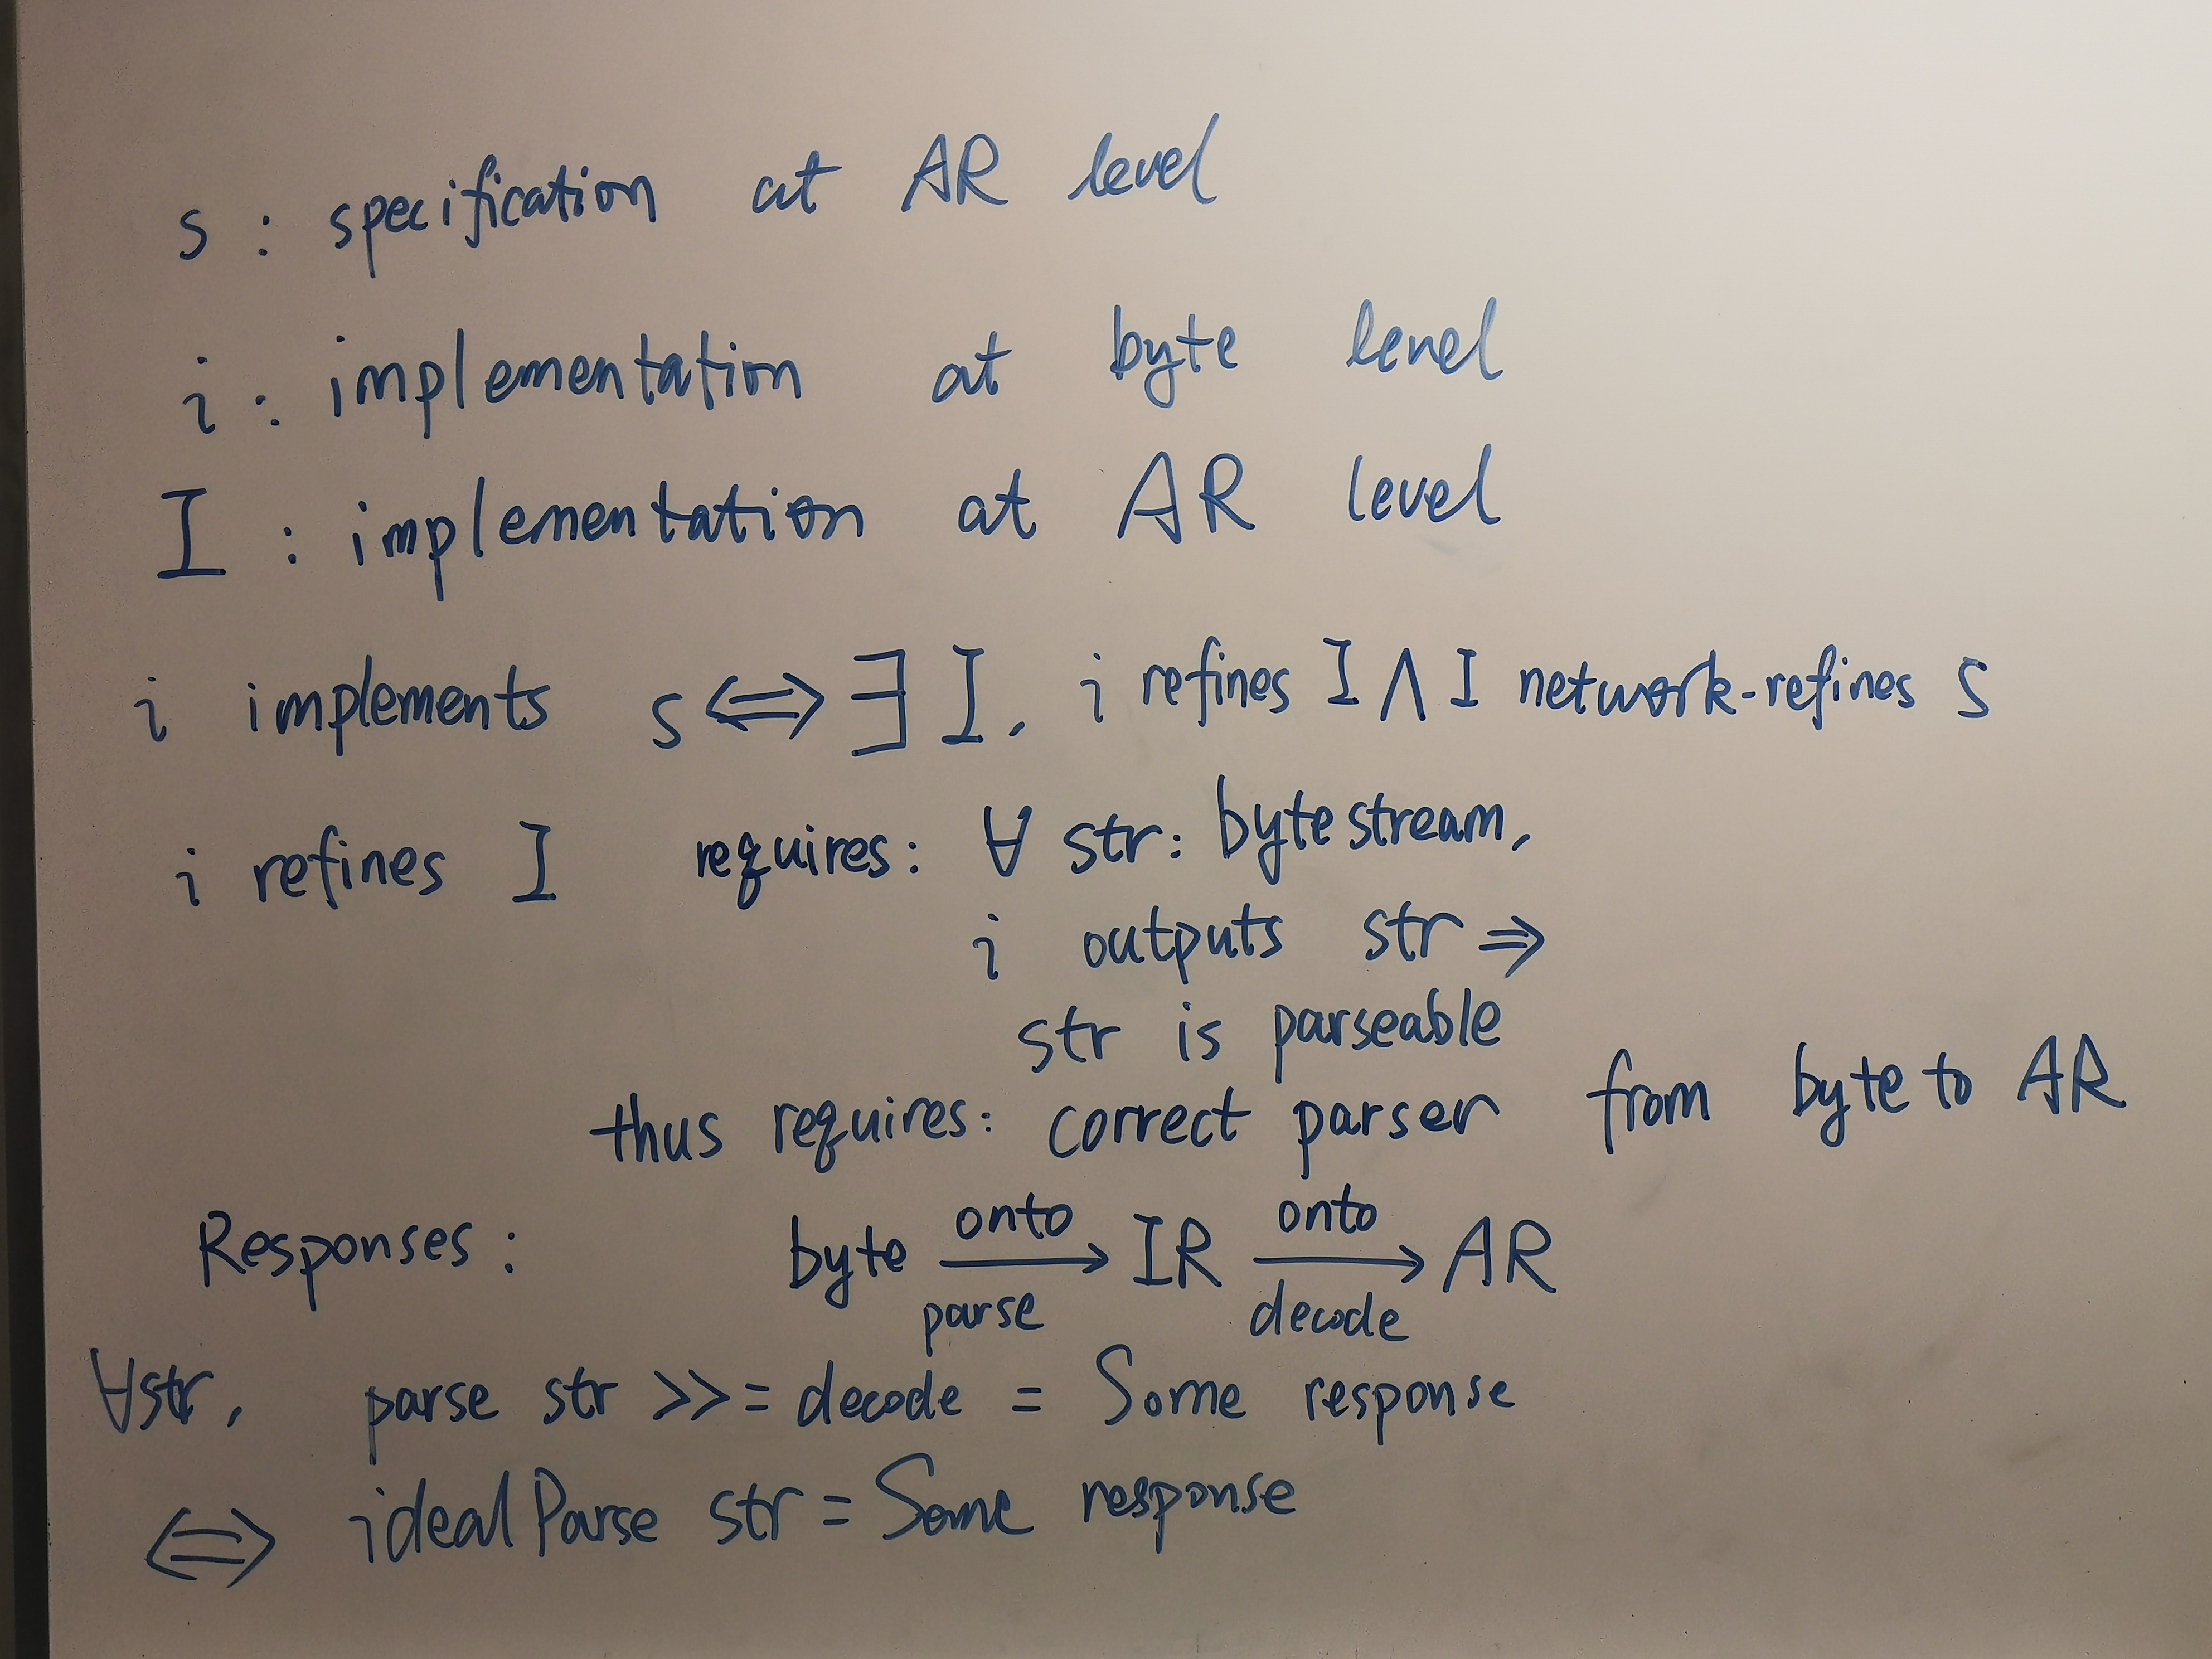
\includegraphics[width=\textwidth]{figures/ir-parse}
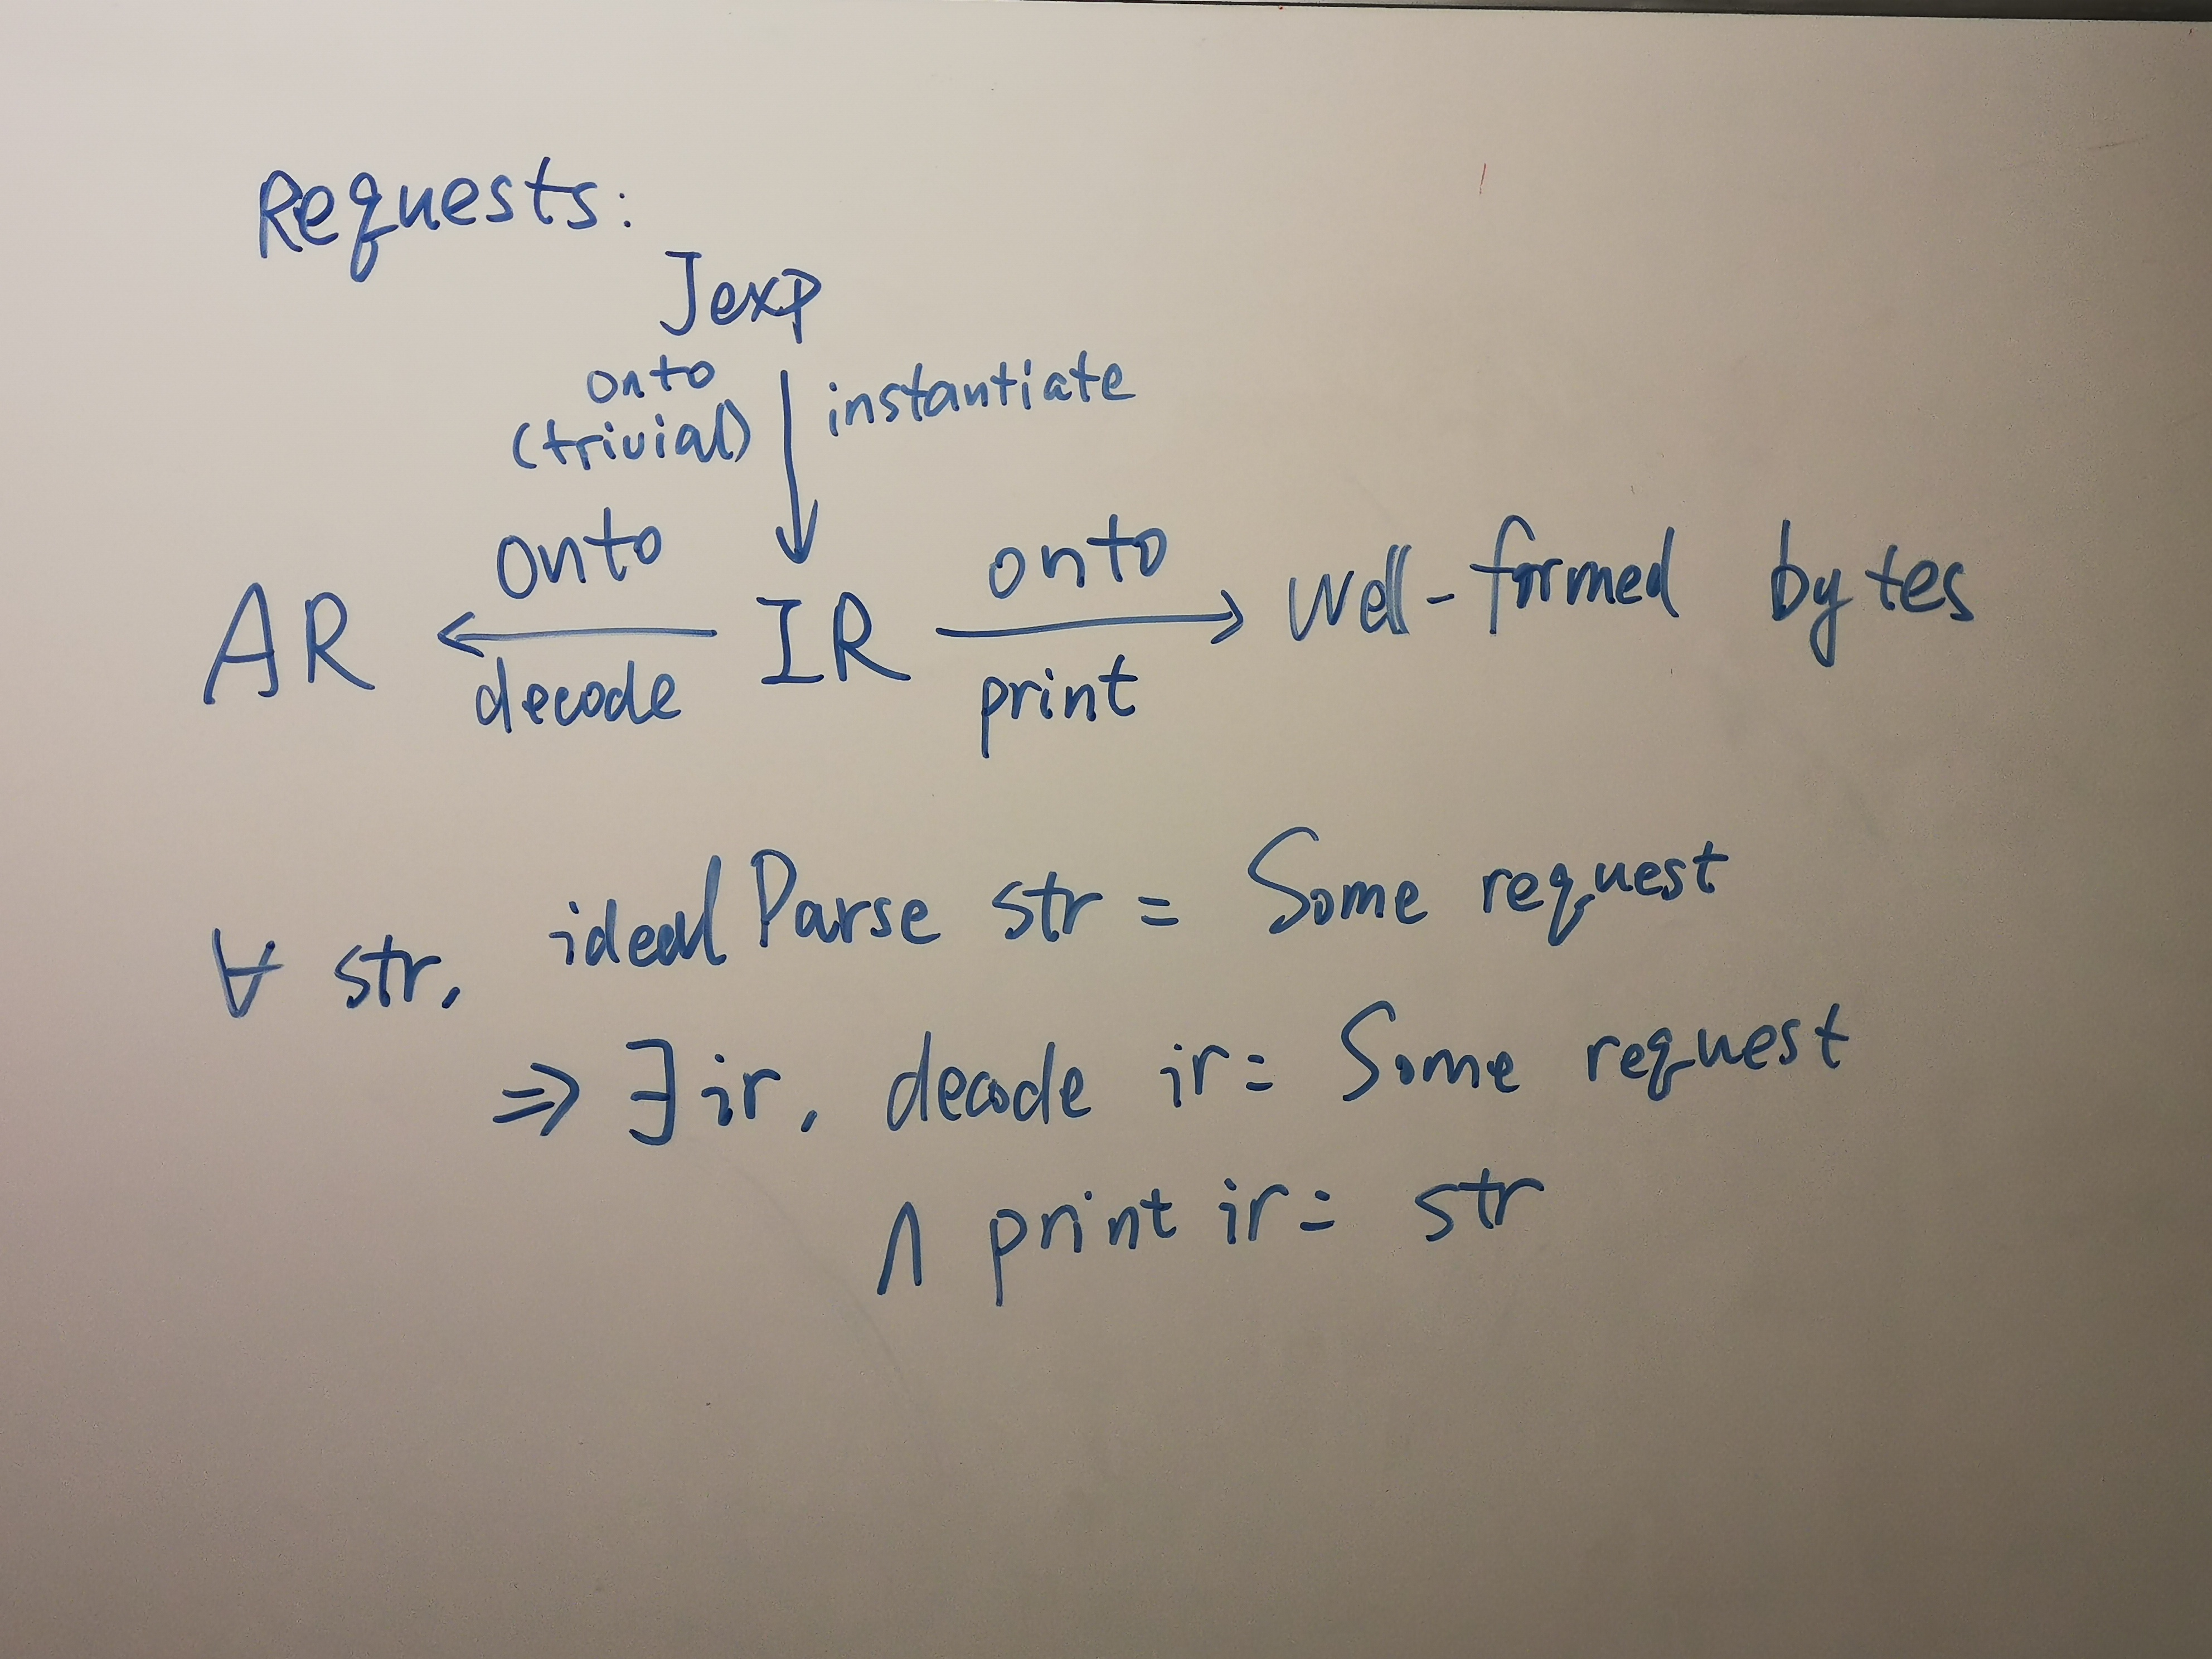
\includegraphics[width=\textwidth]{figures/ir-print}

\subsection{Generic testing library}
Based on my experiments on various web applications, I'll propose a generic
library for specifying application-level protocols.  Developers use the
domain-specific language to define protocol-specific aspects {\it e.g.}
prototype logic, message encoding {\it etc.}  and the library automatically
derives the specification into an interactive tester client that can reveal
servers' incomformance effectively.

5--6+ pages.  Include technical details for evaluation.

Timeline towards dissertation.  Month-level schedule, including publication.

\printbibliography

\end{document}
